\documentclass[letterpaper,14pt,oneside]{report}
\usepackage{amssymb,amsmath,alltt}
\usepackage{graphicx}
\usepackage[latin1]{inputenc}
\usepackage[spanish]{babel}
\usepackage{setspace}
\usepackage{epsfig}
\usepackage{float}
\usepackage[10pt]{moresize}
\usepackage{titlesec}

%este es el archivo de configuracion
\usepackage{fancyhdr}
\usepackage[includeheadfoot,footskip=.5cm]{geometry}
\usepackage[small,bf]{caption}
%\usepackage{mathtools}
\usepackage{multirow}
\usepackage{array}
\usepackage{color, colortbl}
%
\pagestyle{fancy}
\geometry{lmargin=2cm,rmargin=3cm,tmargin=0.5cm,bmargin=4cm}
\def\arraystretch{1.5}

% Coloca una línea en los encabezados
\fancyhf{}
\fancyhead[L]{}
\fancyhead[R]{}
\fancyhead[C]{
	\begin{table}[H]
		\centering
		\begin{tabular}{ p{4.5cm} c p{1.6cm} }
		\multirow{3}{*}{
			
\includegraphics[width=0.25\textwidth]{images/logoecci.png}}
		 & ESCUELA COLOMBIANA DE CARRERAS INDUSTRIALES & \\
		 & GERENCIA DE PROYECTOS &\\
		 & &\hfill {\footnotesize GESPRO07}\\
		\end{tabular}
	\end{table}
}
% para mostrar el paginado
\fancyfoot[R]{\thepage}
\renewcommand{\headrulewidth}{0cm}
% Cambia la estructura de una página en blanco
\fancypagestyle{plain}{
\fancyhead[L]{}
\fancyhead[R]{}
\fancyhead[C]{
	\begin{table}[H]
		\centering
		\begin{tabular}{ p{4.5cm} c p{1.6cm} }
		\multirow{3}{*}{
			
\includegraphics[width=0.25\textwidth]{images/logoecci.png}}
		 & ESCUELA COLOMBIANA DE CARRERAS INDUSTRIALES & \\
		 & GERENCIA DE PROYECTOS &\\
		 & &\hfill {\footnotesize GESPRO07}\\
		\end{tabular}
	\end{table}
}
\renewcommand{\headrulewidth}{0pt}
}

% Cambia el ancho del encabezado
%\setlength{\headwidth}{16.5cm}

% Cambia el espacio para el encabezado
\setlength{\voffset}{5pt}
\setlength{\headheight}{70pt}
\setlength{\headsep}{0.5cm}

% Cambia el margen de los pies de figura
\setlength{\captionmargin}{10pt}

% Borra la palabra Capítulo del \chaptermark:
\renewcommand{\chaptermark}[1]{\markboth{\MakeUppercase
{\thechapter. #1}}{}}
% Quita la palabra capitulo
\addto\captionsspanish{\renewcommand{\chaptername}{}}

%definicion de colores
\definecolor{LightGrey}{gray}{0.9}
\definecolor{lgray}{gray}{0.75}
\definecolor{Grey}{gray}{0.7}

% Definiendo tamanos de los titulos
\titleformat{\chapter}
	{\bfseries\normalfont\normalfont}
	{\thechapter.}
	{6pt}
	{}
\titlespacing*{\chapter}{0pt}{0pt}{0pt}

\titleformat{\section}[block]
	{\Large\normalfont}
	{\thesection.}
	{6pt}
	{}
\titlespacing*{\section}{0pt}{0pt}{0pt}

\titleformat{\subsection}
{\normalfont\large\bfseries}{\thesubsection}{12pt}{}
\titleformat{\subsubsection}
{\normalfont\normalsize\bfseries}{\thesubsubsection}{12pt}{}
\titleformat{\paragraph}[runin]
{\normalfont\normalsize\bfseries}{\theparagraph}{12pt}{}
\titleformat{\subparagraph}[runin]
{\normalfont\normalsize\bfseries}{\thesubparagraph}{12pt}{}

%definiendo el modo de insercion de capitulos
\titleclass{\chapter}{top}

%definicion de recuadros gris y texto negro para secciones y capitulos
\titleformat{\chapter}[hang]{\Large\normalfont}{%
}{0em}{%
    {%
        \setlength{\fboxsep}{0pt}%
        \colorbox{lgray}{\makebox[\textwidth]{\Large\strut}}%
    }%
    \hspace*{-\textwidth}%
        {\thechapter}%
        \hspace*{1em}%
}[]
%
%\titleformat{\section}[hang]{\Large\normalfont}{6pt}{%
%    {%
%        \setlength{\fboxsep}{0pt}%
%        \colorbox{lgray}{\makebox[\textwidth]{\Large\strut}}%
%    }%
%    \hspace*{-\textwidth}%
%        {\thesection}%
%        \hspace*{1em}%
%}[]

% Se puede cambiar los siguientes parámetros para modificar el acomodo del texto
\parskip= 6pt
%definicion de los archivos

\begin{document}
\pagenumbering{arabic} \setcounter{page}{1}
\pagestyle{fancy}

{\let\clearpage\relax\par%
\begin{table}[H]
	\centering
	\begin{tabular}{| c | c | c | c | p{1.5cm} | p{3cm} | }
	\hline
	\rowcolor{Grey}
	\multicolumn{6}{c}{CONTROL DE VERSIONES} \\
	\cline{1-6}\noalign{\smallskip}
	\hline
	\rowcolor{LightGrey}
	Versi\'on & Hecha por & Revisada por & Aprobada por & Fecha & Motivo \\ \hline
	1.0 & Javier Serrano & Yeymi Gonz\'alez & Jenny Fierro & Febrero 22 de 2015 & Creaci\'on de formato \\
	\hline
	2.0 & Javier Serrano & Yeymi Gonz\'alez & Jenny Fierro & Abril 10 de 2015 & Correciones para \newline segunda entrega \\
	\hline
	
	\end{tabular}
\end{table}
%}
{\let\clearpage\relax\par\chapter{Apreciaciones generales.}
%
Las conclusiones se basan en el an\'alisis tomado de la matriz de asociaci\'on de poder e inter\'es 
(\ref{matrizstakeholders}), resultado de la encuesta realizada a los stakeholders involucrados (GESPRO04 - Registro 
de Stakeholders.pdf) en el proyecto (GESPRO05 - Encuesta y Matriz.pdf).\\
%
\begin{figure}[H]
    \centering
    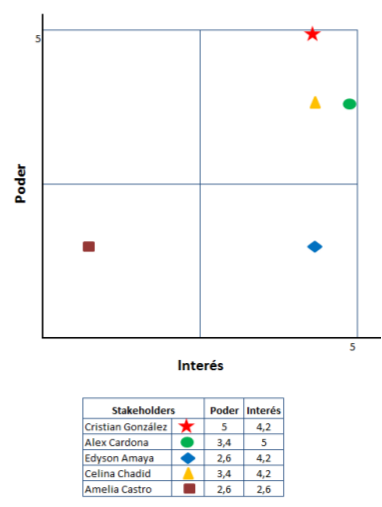
\includegraphics[width=0.95\textwidth]{images/matrizstakeholders.png}
    \caption{Matriz de clasificaci\'on de Stakeholders.}
    \label{matrizstakeholders}
\end{figure}
%
\chapter{STAKEHOLDERS}
%
\section{Cristian Gonz\'alez}
%
\noindent \textbf{Cargo:} Gerente General.\\
%
\textbf{Calificaci\'on poder:} 5.0\\
%
\textbf{Calificaci\'on inter\'es:} 4.2\\
%
\textbf{Impacto:} Alto.\\
%
\textbf{Conclusiones:}\\
%
\\Debido al rol que desempe\~na, es la persona con m\'as poder sobre la organizaci\'on; es el encargado
de la autorizaci\'on de adquisiciones y compras. Por otra parte, a diferencia de otros casos, tiene mucho 
inter\'es en la implementaci\'on de este proyecto, dado que le afecta directamente para la toma de decisiones
y la elaboraci\'on de planes estrat\'egicos dentro de la organizaci\'on.\\
%
\section{Alex Cardona}
%
\noindent \textbf{Cargo:} Gerente Administrativo y financiero.\\
%
\textbf{Calificaci\'on poder:} 3.4\\
%
\textbf{Calificaci\'on inter\'es:} 5.0\\
%
\textbf{Impacto:} Alto.\\
%
\textbf{Conclusiones:}\\
%
\\Aunque no posea voto en la toma de decisiones, su impacto afecta el proyecto debido a que su rol es indispensable
en el acompa\~namiento para la elaboraci\'on de los planes estrat\'egicos y por eso, es que demuestra gran
inter\'es en la implementaci\'on del mismo. Se recomienda tener en cuenta de forma particular todas sus 
inquietudes.\\
%
\section{Edyson Amaya}
%
\noindent \textbf{Cargo:} Gerente de producci\'on.\\
%
\textbf{Calificaci\'on poder:} 2.6\\
%
\textbf{Calificaci\'on inter\'es:} 4.2\\
%
\textbf{Impacto:} Medio.\\
%
\textbf{Conclusiones:}\\
%
\\Aunque no posea voto en la toma de decisiones, su impacto afecta el proyecto debido a que su rol es indispensable
en el acompa\~namiento para la elaboraci\'on de los planes estrat\'egicos y por eso, es que demuestra gran
inter\'es en la implementaci\'on del mismo. Se recomienda tener en cuenta de forma particular todas sus 
inquietudes.\\
%
\section{Celina Chadid}
%
\noindent \textbf{Cargo:} Gerente de recursos humanos.\\
%
\textbf{Calificaci\'on poder:} 3.4\\
%
\textbf{Calificaci\'on inter\'es:} 4.2\\
%
\textbf{Impacto:} Alto.\\
%
\textbf{Conclusiones:}\\
%
\\Aunque no posea voto en la toma de decisiones, su impacto afecta el proyecto debido a que su rol es indispensable
en el acompa\~namiento para la elaboraci\'on de los planes estrat\'egicos y por eso, es que demuestra gran
inter\'es en la implementaci\'on del mismo. Se recomienda tener en cuenta de forma particular todas sus 
inquietudes.\\
%
\section{Amelia Castro}
%
\noindent \textbf{Cargo:} Gerente comercial.\\
%
\textbf{Calificaci\'on poder:} 2.6\\
%
\textbf{Calificaci\'on inter\'es:} 2.6\\
%
\textbf{Impacto:} Bajo.\\
%
\textbf{Conclusiones:}\\
%
\\Su rol no implica voz ni voto en la toma de decisiones a nivel gerencial; su compromiso con los planes
estrat\'egicos est\'a al mismo nivel que el de todos en la empresa: comprometidos en la colaboraci\'on general.
Su nivel de inter\'es sobre el proyecto es bajo porque no requiere muchas de las funcionalidades ofrecidas.\\}

\end{document}
